% -*- mode: fundamental -*-

% ****************************************************************

\chapter{BSV: Packages, Files and Imports; Importing C code}

\markboth{Ch \arabic{chapter}: BSV: Packages}{\copyrightnotice}

\setcounter{page}{1}
% \renewcommand{\thepage}{\arabic{page}}
\renewcommand{\thepage}{\arabic{chapter}-\arabic{page}}

\label{ch_Packages}

% ****************************************************************

\section{Introduction}

In this chapter we describe the BSV facilities for managing large BSV
programs: organizing them into separately compilable packages,
controlling which entities in a package are visible outside the
package (exports), and referring from one package to entities defined
in another package (imports).

We will also describe how we can import C code for use by BSV.

% ****************************************************************

\section{Packages and files}

\index{BSV!package@{\tt package}}
\index{BSV!endpackage@{\tt endpackage}}

Like many programming languages, BSV has facilities to organize large
programs into separately compilable, meaningful, reusable parts.  A
BSV program may be organized into one or more \emph{files} or
\emph{packages}.  This is illustrated in
Figure~\ref{Fig_BSV_program_structure}.
\begin{figure}[htbp]
  \centerline{\includegraphics[width=6in,angle=0]{Figures/Fig_BSV_program_structure}}
  \caption{\label{Fig_BSV_program_structure}
           File-level view of a BSV program}
\end{figure}

A package can contain a number of top-level statements (more detail
about this in Section~\ref{Sec_package_contents}).  One kind of
top-level statment is the ``\verb|import|'' statement, illustrated in
the diagram.  This allows an importing package $p_1$ to use all the
identifiers exported by a package $p_2$ (in addition to indentifiers
defined in $p_1$ itself).

There is a one-to-one correspondence between files and packages.  In
each import statements in the diagram we provide a package name $p$;
the \emph{bsc} compiler uses the imported package name $p$ to find a
file called $p$\verb|.bsv| containing the definition of package $p$.

% ****************************************************************

\section{What's in a Package?}

\label{Sec_package_contents}

Figure~\ref{Fig_BSV_Package} illustrates the typical
structure and contents of a package/file.
\begin{figure}[htbp]
  \centerline{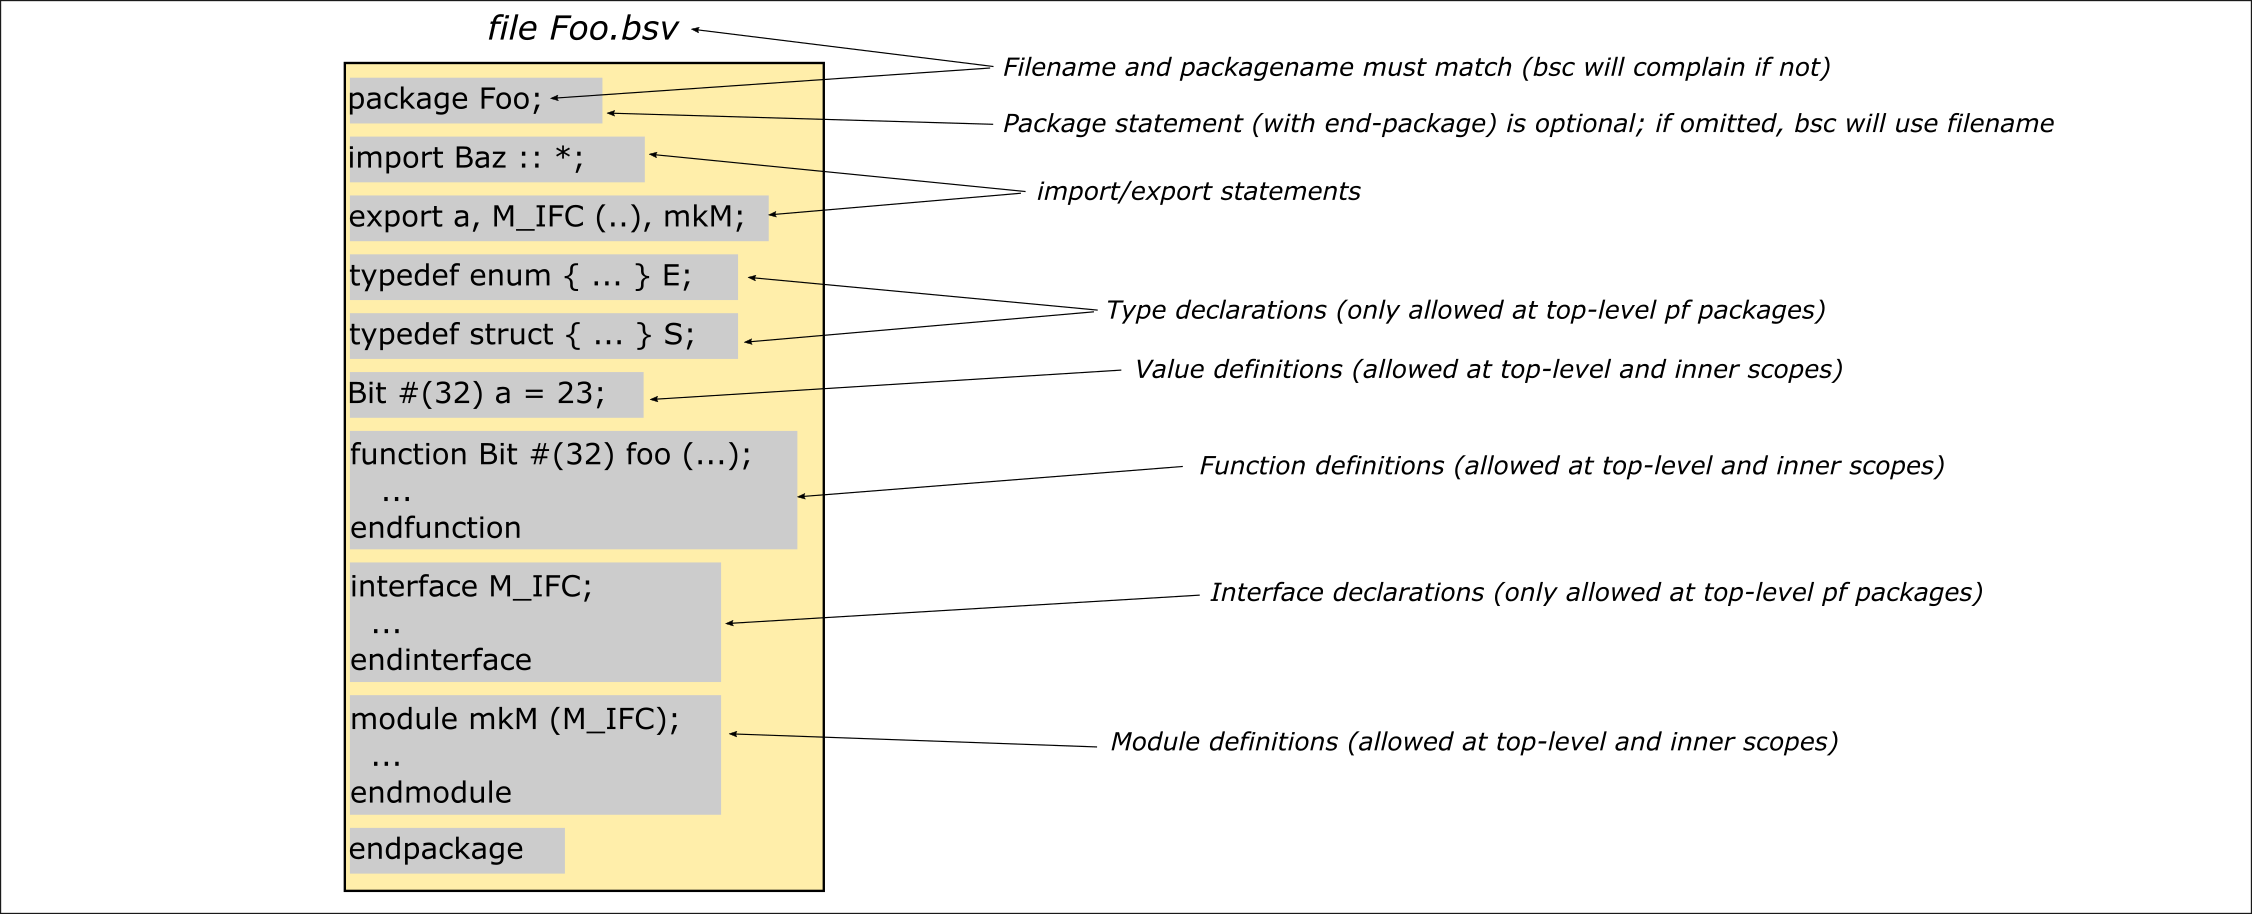
\includegraphics[width=6in,angle=0]{Figures/Fig_BSV_Package}}
  \caption{\label{Fig_BSV_Package}
           What's in a BSV package/file?}
\end{figure}

The \verb|package|--\verb|endpackage| brackets---the first and last
lines of the file---are optional; if omitted, the \emph{bsc} compiler
will implicitly create a package name using the file name.  We
recommend always to use \verb|package|--\verb|endpackage|, except
perhaps for small, experimental, one-off programs to test some small
concept.

At the top-level of a package we find import/export statements, type
declarations, value definitions, function definitions interface
declarations and module definitions.

Import/export statements and type and interface declarations are only
allowed at the top-level of a package and not inside any nested
scopes.  An interface declaration is just a kind of type declaration;
its declared interface identifier is used just like a type.

Value, function and module definitions appear at package top-level,
but can also be inside nested scopes (inside function and module
definitions, or other local scopes like \verb|begin|--\verb|end| and
\verb|action|--\verb|endaction| blocks).  Function and module
definitions are, in fact, just value definitions of functional and
module type, respectively.

The top-to-bottom order of entities in a package is not important,
just that if an entity $x$ is defined in the package and used by
another entity $y$ in the same package, then $x$ should be given
before $y$.  We typically place import/export statements at the top of
the file.

Each package/file is separately compiled by the \emph{bsc} compiler,
which saves information about the compilation so that it won't be
recompiled unless the source file has subsequently been modified.

% ****************************************************************

\section{Visibility of names, exports and imports}

The \verb|package|, \verb|import| and \verb|export| statements work
just like in SystemVerilog (in fact, using the same syntax).  The
\verb|export| and \verb|import| statements control visibility of names
across packages.  This is illustrated in Figure~\ref{Fig_BSV_namespace_control}.
\begin{figure}[htbp]
  \centerline{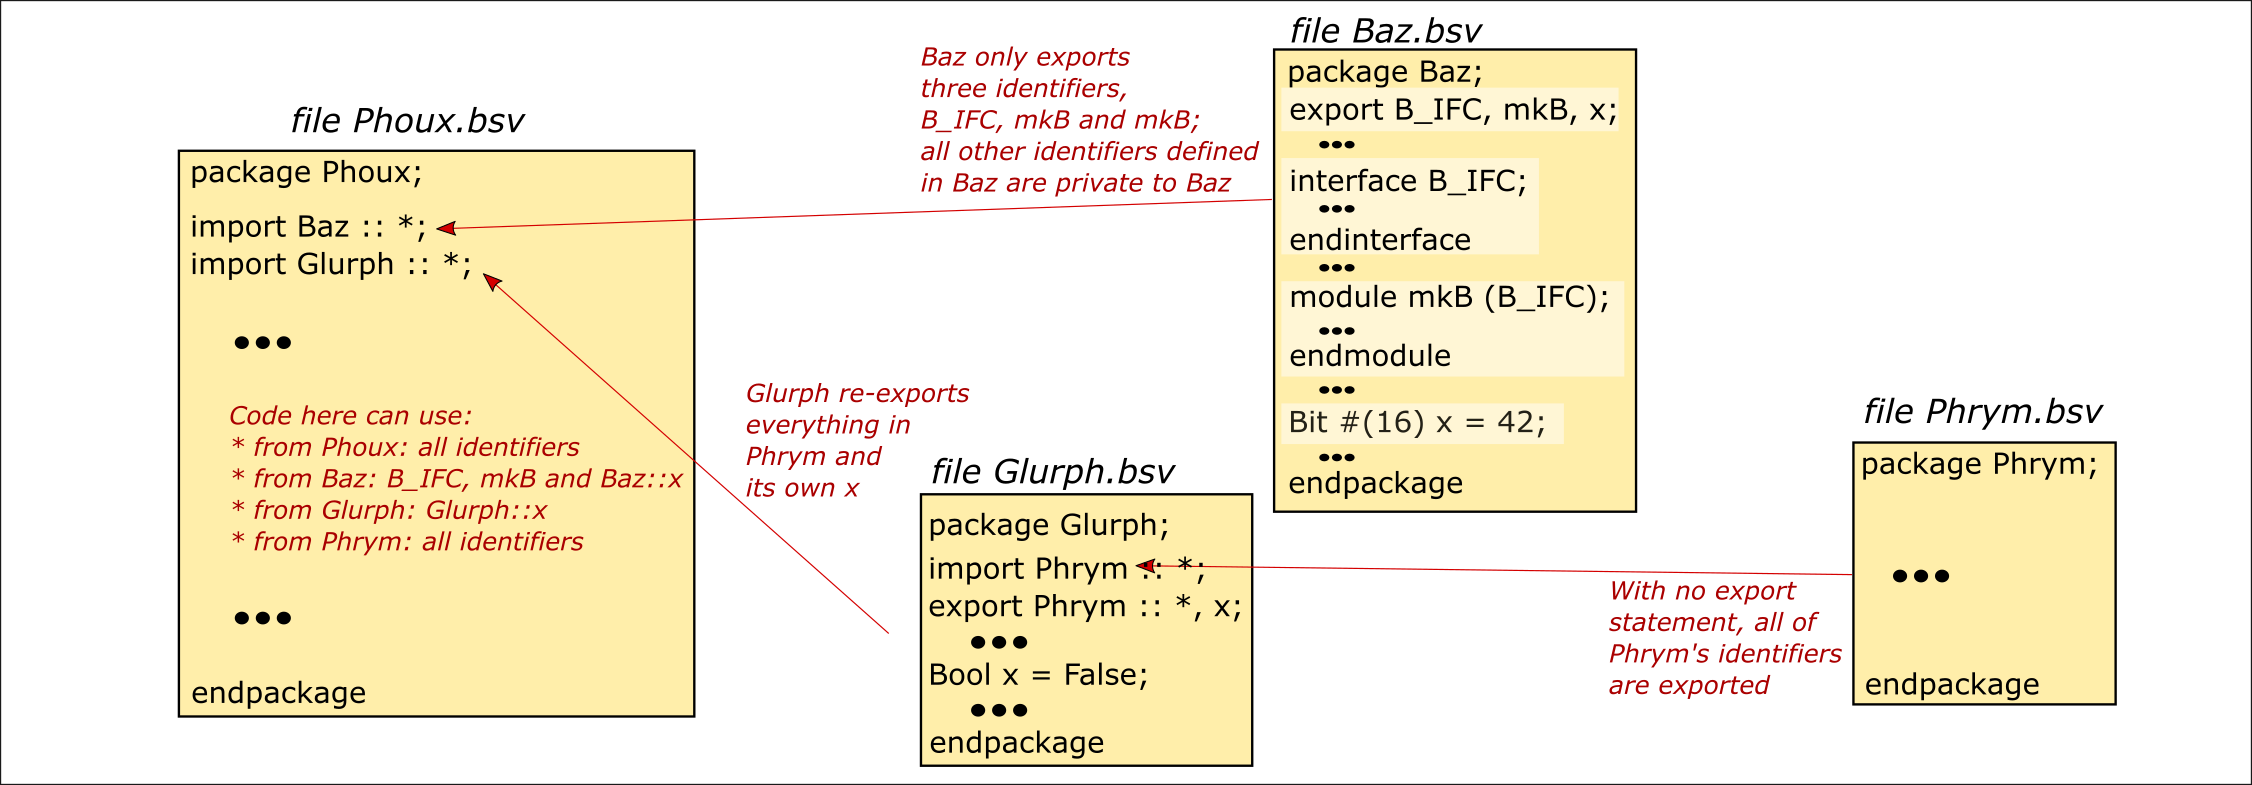
\includegraphics[width=6in,angle=0]{Figures/Fig_BSV_namespace_control}}
  \caption{\label{Fig_BSV_namespace_control}
           Namespace control with imports and exports}
\end{figure}

\index{BSV!export@{\tt export} statement}
\index{BSV!import@{\tt export} statement}

A package \verb|P| that defines a name $x$ can make it visible outside
using an \verb|export| statement.  As a shorthand, if there is no
\verb|export| statement, then \emph{all} the names defined in a
package are made visible outside.  For convenient readability, if
there are many explicitly exported names, they can be provided using
multiple \verb|export| statements.

A package \verb|Glurph| can also \emph{re-export} names it has
imported from some other package \verb|Phrym|.

If a package \verb|Phoux| needs to use a name \verb|x| defined in some
other package \verb|Baz|, it must explicitly ``\verb|import|'' the
package with the syntax:

{\small
\begin{Verbatim}[frame=single, numbers=left]
import Baz :: *;
\end{Verbatim}
}

which makes all the names exported by \verb|Baz| available for use in
\verb|Phoux|.

% ----------------
\vspace{2ex}

NOTE:
\fbox{\small
\begin{minipage}{5in}

In SystemVerilog, in {\tt import} statement, instead of ``{\tt *}''
one can list just the names actually needed, one does not have to
import all the names exported by another package.  This selective
import is not currently supported in BSV.

\end{minipage}}
% ----------------

% ================================================================

\subsection{Resolving ambiguous imports}

\index{BSV!Fully-qualified imported names}

If a package \verb|Phoux| imports two other packages \verb|Baz| and
\verb|Glurph|, and both those packages define an identifier \verb|x|,
then the identifier \verb|x| is ambiguous in \verb|Phoux|.  This can
always be resolved by replacing any use of \verb|x| in \verb|Phoux| by
a so-called \emph{fully qualified name}, \verb|Baz::x| or
\verb|Glurph::x| to identify exactly which \verb|x| is intended.

% ================================================================

\subsection{Exporting types abstractly}

\index{BSV!Exporting types abstractly}

When exporting a struct type \verb|S| or enum type \verb|E| using
\verb|export|, there is a difference between these two ways of
exporting:

\begin{center}
 \begin{tabular}{ccc}
  {\tt export S (..);} & \hmm {\vs} \hmm & {\tt export S;} \\
  {\tt export E (..);} & \hmm {\vs} \hmm & {\tt export E;}
 \end{tabular}
\end{center}

In the versions on the left the field names of the struct and the
labels of the enum are also made visible; on the right, they are not.
The latter case useful in defining a so-called ``\emph{abtract data
type}'', {\ie} a type that is known outside the package but whose
internal details are hidden.

Since an interface is just like a struct type, if we explicitly export
it we typically use:

\begin{center}
\mbox{\tt export M\_IFC (..);}
\end{center}

since we normally want all the interface methods in the interface to
be visible.

% ****************************************************************

\section{Importing C/C++ functions into BSV simulations}

\index{BSV!Importing C and C++ functions}

% ----------------
\vspace{2ex}

NOTE:
\fbox{\small
\begin{minipage}{5in}

In Drum and Fife code, this BSV feature is only used in the testbench,
specifically the Memory System attached to the CPU.  This section can
be ignored if that topic is not of interest.

\end{minipage}}
% ----------------

\vspace{1ex}

There are many reasons to import C functions into BSV simulations
(whether Verilog simulation or Bluesim simulation):

\begin{itemize}

 \item Many applications begin life as a C/C++ model, such as a C/C++
       algorithm that we are trying to accelerate in hardware, or an
       algorithm that we are still prototyping in C/C++ while
       developing the rest of the system.

 \item C/C++ is useful for testbench components: They will run much
       faster than Verilog simulation, and so will not be a
       performance burden on simulating the Verilog of interest.  They
       have full-service access to data files and operating-system
       services.

\end{itemize}

A C function can be imported into BSV with the simple steps described
in the next sections.

BSV can only import C functions.  If you need to import a C++
function, write a C wrapper function that is invoked by BSV; that C
function can then invoke your C++ function.

An imported C function invoked in BSV is semantically instantaneous,
never a temporal process.  It is imported with \verb|Action| or
\verb|ActionValue| type or a pure (combinational) type.\footnote{Of
course an invoked C function, before it returns, could start a C
``pthread'' which then runs concurrently with the BSV simulation.}

% ================================================================

\subsection{In the BSV code declare a BSV version of the C function}

\index{BSV!import "BDPI"@{\tt import "BDPI"}}

In the BSV code, the imported C function will be invoked exactly like
a normal BSV function.  We declare the header of this ``BSV'' function
({\ie} just the result type, function name and arguments with their
types, and not the function body), preceded by the phrase {\tt import
"BDPI"}:

\begin{center}
 \fbox{\small
  \begin{minipage}{5in}
   \begin{tabbing}
   {\tt import "BDPI"} \\
   {\tt function} \hm \emph{BSV-type} \hm \emph{function-name (} \= \emph{BSV-type \hm arg} \\
                                                                 \> ... \\
                                                                 \> \emph{BSV-type \hm arg} {\tt );}
   \end{tabbing}
  \end{minipage}
 }
\end{center}

The argument- and result-passing conventions are simple, adjusting for
the C's limitation that arguments and results be can at most 64-bits
wide:

\begin{itemize}

 \item BSV values of sizes up to 8, 16, 32 or 64 bits are passed as
       arguments and results of C type \verb|uint8_t|,
       \verb|uint16_t|, \verb|uint32_t| and \verb|uint64_t|,
       respectively, for both arguments and results, in the same
       corresponding positions.

 \item For a BSV argument value of size greater than 64 bits, it is
       passed to C as a pointer to memory containing the BSV value.

 \item For a BSV \emph{result value} of size greater than 64 bits, the
       corresponding C function prototype changes slightly:

       \begin{tightlist}

        \item It gains an extra first argument which gets a pointer to
              memory which should be filled by the C function with the
              BSV value to be returned.

        \item Because of this, it has a \verb|void| return type.

       \end{tightlist}
\end{itemize}

% ================================================================

\subsection{Compile the BSV code with the \emph{bsc} compiler}

If you are compiling for Bluesim, there is no change to how you invoke
\emph{bsc}.

If you are compiling to Verilog, provide the additional flag
``\verb|-use-dpi|'' on the command line.  This will generate standard
SystemVerilog \verb|import "DPI-C"| declarations in the generated
Verilog.

% ================================================================

\subsection{Linking}

For Bluesim linking, simply provide the C file(s) implementing
imported C functions as an additional command-line arguments to
\emph{bsc}.

For Verilog linking, in the imported C code we recommend adding the
following for each of the imported C functions:

{\small
\begin{Verbatim}[frame=single, numbers=left]
#ifdef __cplusplus
// 'C' linkage is necessary for linking with Verilator object files
extern "C" {
    ... imported C function's prototype ...
}
#endif
\end{Verbatim}
}

This directs the C/C++ compiler to compile the C function with C
argument-passing conventions instead of C++ argument passing, which is
necessary for SystemVerilog DPI-C.  Verilog simulator tools like
Verilator compile the C code with a C++ compiler which, by default,
would use C++ argument-passing.

For Verilator linking, simply provide the C/C++ file(s) implementing
the imported C functions as additional arguments to the
\verb|verilator| command.

For other Verilog simulators, the linking details may vary; please
consult their respective manuals or experts on how to link-in C code
under the SystemVerilog DPI-C standard.

% ================================================================

\subsection{Recommendations for arguments and results of imported C/C++ functions}

These recommendations circumvent potential complications when using
imported C code in BSV.

% ----------------------------------------------------------------

\subsubsection{Only use BSV types corresponding to C types}

The data passed between BSV and C have the standard BSV packed
representations in bits.  It can be tricky in C to deal with, say, a
BSV 13-bit value that, in C, is a \verb|uint16_t|.  We recommend only
using BSV arguments/results whose sizes are multiples of 8-bits so
that they map exactly to bytes in C.

Even for BSV structs and vectors, only use structs and vectors whose
elements are 8-bit byte-sized.  Accessing/updating the components in C
is vastly easier with these constraints.

If an original BSV type $T$ does not have ``byte-aligned'' components,
we often define a new type $T2$ with byte-aligned components and copy
values from $T$ to $T2$ before the call (for arguments) or from $T2$
to $T$ (for results).  These is extra, technically unnecessary
``copying'' of data, but the resulting simplification of the C code is
well worth it.

For structs, be careful that C structs may have ``gaps'' or
``padding'' between fields to improve word-alignment, whereas BSV
structs are tightly packed.  Thus a BSV struct and a C struct, though
they may look identical, may have different data representations.

% ----------------------------------------------------------------

\subsubsection{Use {\tt ActionValue\#(t)} for imported C function's result}

In an \verb|import "BDPI"| declaration the type of the result the
function may be \verb|Action|, or \verb|ActionValue#(t)| or some type
$t$.  As discussed in Section~\ref{Sec_Pure_vs_Side_Effect_functions},
in BSV the last case (not an action or actionvalue) is taken as a
strong guarantee of mathematical purity (and absence of side-effects);
the \verb|bsc| compiler may merge multiple invocations that have the
same arguments, and it may move a function elsewhere in the code with
different control conditions.  These optimizations can lead to nasty
surprises when the C function is not really pure (including core-dumps
if it relies on prior initializations).

We recommend normally using \verb|ActionValue#(t)| for the result of
any imported C function (or \verb|Action| if the C result is
\verb|void|) to avoid surprises.

Use a non-action/actionvalue return type \emph{only} if you are
absolutely sure that the C function is pure and does not need any
other initializations before invocation ({\eg} the C library
\verb|toupper| character transfomer or \verb|cos()| trigonometric
function).  Even for these, be safe and use an actionvalue function.

% ================================================================

\subsection{Example: Memory Model for Drum and Fife}

For Fife and Drum, because our focus is on the CPU module, we
implement the memory system in C for convenience.  In addition to the
speed reason (not slowing down simulation), C is also more convenient
for reading in memhex32 and ELF files.

\input{Code_Extracts/Mems_Devices}

The corresponding C function prototype, in a C file is:

{\small
\begin{Verbatim}[frame=single, numbers=left]
#ifdef __cplusplus
// 'C' linkage is necessary for linking with Verilator object files
extern "C" {
void c_mems_devices_req_rsp (uint8_t        *result_p,
			     const uint64_t  inum,
			     const uint32_t  req_type,
			     const uint32_t  req_size_code,
			     const uint64_t  addr,
			     const uint32_t  client,
			     uint8_t        *wdata_p);
}
#endif
\end{Verbatim}
}

% ****************************************************************
